% ====================================================================
% Informe final -- FS3008 Dinámica y estructura de sistemas físicos
% Basado en la plantilla JAES (Journal_of_the_Audio_Engineering_Society_JAES_template.tex)
% Compilar: pdflatex -> bibtex -> pdflatex -> pdflatex  (o latexmk -pdf)
% =====================================================================
\documentclass[fleqn,final]{jaes}
% [final]: sin números de línea ni marca de agua "DRAFT".
% Para revisión con números de línea, cambiar a [fleqn,draft].

% Metadatos
\jyear{noviembre de 2026}
\jmonth{}

% Idioma
\usepackage[spanish,es-tabla,es-nodecimaldot,es-noshorthands]{babel}
\addto\captionsspanish{%
  \renewcommand\figurename{Fig.}%
  \renewcommand\tablename{Tabla}%
  \renewcommand\refname{Referencias}%
  \renewcommand\bibname{Referencias}%
}

% Matemáticas
\usepackage{amsmath}\setlength{\mathindent}{10pt}
% (amssymb no se carga: la clase usa newtxmath, que ya incluye esos símbolos)
\usepackage{bm}

% Marcadores del PDF (evita el aviso "Rerun to get outlines right")
\usepackage{bookmark}

% Figuras: se usan las figuras finales generadas por el código
\graphicspath{{../figuras/}}
% Colocación de figuras en dos columnas: permitir más figuras por página
\usepackage{placeins}
\usepackage{stfloats}% figuras anchas también abajo
\setcounter{topnumber}{3}
\setcounter{dbltopnumber}{3}
\renewcommand{\topfraction}{0.9}
\renewcommand{\dbltopfraction}{0.9}
\renewcommand{\textfraction}{0.07}
\renewcommand{\floatpagefraction}{0.8}
\renewcommand{\dblfloatpagefraction}{0.8}

% Referencias cruzadas (en español)
\usepackage[capitalise]{cleveref}
  \crefname{equation}{Ec.}{Ecs.}
  \Crefname{equation}{Ec.}{Ecs.}
  \crefformat{section}{\textsc{Sec.~#2#1#3}}
  \Crefformat{section}{\textsc{Sec.~#2#1#3}}
  \crefformat{figure}{{Fig.~#2#1#3}}
  \Crefformat{figure}{{Fig.~#2#1#3}}
  \crefformat{table}{{Tabla~#2#1#3}}
  \Crefformat{table}{{Tabla~#2#1#3}}

% Palabras clave en español (la clase imprime "Keywords:")
\makeatletter
\renewenvironment{keywords}{\par\addvspace{11pt}
  \noindent\textbf{Palabras clave: }\keywordsfont\ignorespaces}{\par\addvspace{0pt}}
\makeatother

% Encabezados y pies de página (la clase trae textos de la revista JAES)
\renewcommand*\JAESHeaderText{UNIVERSIDAD EAFIT}
\makeatletter
\def\@jname{FS3008 Dinámica y estructura de sistemas físicos}
\newcommand{\jaespie}[1]{\makebox[\textwidth][s]{\rhfont#1}}
% Primera página: sin la palabra "DRAFT"
\def\ps@plain{\let\@mkboth\@gobbletwo%
  \def\@evenhead{}\def\@oddhead{}%
  \def\@evenfoot{\jaespie{\thepage\hfill\@jname, \@jyear}}%
  \def\@oddfoot{\jaespie{\@jname, \@jyear\hfill\thepage}}}
\def\ps@headings{%
  \def\@evenhead{{\rhfont\jaes@leftmark}\hfil{\rhfont\JAESHeaderText}}%
  \def\@oddhead{{\rhfont\JAESHeaderText}\hfil{\rhfont\jaes@rightmark}}%
  \def\@evenfoot{\jaespie{\thepage\hfill\@jname, \@jyear}}%
  \def\@oddfoot{\jaespie{\@jname, \@jyear\hfill\thepage}}}
% Sin sección de biografías de autores ("THE AUTHORS"): el curso no la pide
\def\printbiography{}
\makeatother

% Unidades usadas en el proyecto
\newcommand{\um}{\,\mu\mathrm{m}}
\newcommand{\uN}{\,\mu\mathrm{N}}

\begin{document}

% ---------------------------------------------------------------------
% Título
% ---------------------------------------------------------------------
\title{Influencia de la Configuración Geométrica de una Telaraña Orbicular en su Dinámica Vibratoria Mediante un Modelo de Mecánica Analítica}

% Encabezados de página {Autores}{Título corto, máx. 60 caracteres}
\markboth{HOYOS, RODRÍGUEZ Y LEÓN}{GEOMETRÍA Y DINÁMICA VIBRATORIA DE UNA TELARAÑA}

% ---------------------------------------------------------------------
% Autores
% ---------------------------------------------------------------------
\authorgroup{
\author{AMELIA HOYOS VÉLEZ,}
\author{NICOLLE RODRÍGUEZ ESTUPIÑÁN}
Y \author{MIGUEL ÁNGEL LEÓN BOTERO}
% \email{(correo1)\quad (correo2)\quad (correo3)}   % TODO: correos institucionales, si se quieren incluir
\affil{Ingeniería Física, Escuela de Ciencias e Ingeniería, Universidad EAFIT, Medellín, Colombia}
}

% ---------------------------------------------------------------------
% Resumen (un solo párrafo, sin citas)
% ---------------------------------------------------------------------
\abstract{%
Las arañas orbitelares localizan a sus presas por las vibraciones que llegan por los hilos de su telaraña. Se modela una red de \textit{Araneus diadematus} como masas concentradas unidas por hilos pretensados y, con el formalismo lagrangiano, se obtienen sus ecuaciones de movimiento linealizadas; se demuestra que el problema está bien planteado y que los movimientos transversal y en el plano se desacoplan de forma exacta. Con el modelo, verificado numéricamente, se calculan los modos normales, la respuesta a la caída de una presa y la transmisión de la señal entre nodos para distintas geometrías. La masa de la araña produce un modo de rebote a 2.55~Hz que domina la baja frecuencia; la dirección de la presa se distingue entre 5 y 30~Hz a partir de unos 2~cm del centro, y el número de radiales es el parámetro geométrico más influyente, porque cambia las pretensiones que exige el equilibrio.}
\maketitle

\begin{keywords}
Análisis modal, Arañas orbitelares, Rigidez geométrica
\end{keywords}

% =====================================================================
\section{Introducción}\label{sec:intro}
% =====================================================================

Las arañas orbitelares, como la \textit{Araneus diadematus}, construyen redes
con dos tipos de hilo: los \emph{radiales}, que salen del centro de la red,
el \emph{hub}, hacia el marco, y la \emph{espiral}, un hilo que da
vueltas alrededor del centro y se une a cada radial al cruzarlo; cada
vuelta de la espiral forma un \emph{anillo}
(\cref{fig:geometria}). Además de atrapar presas, la red funciona como
un sensor táctil para la araña: cuando un insecto queda atrapado, sus movimientos generan
vibraciones que viajan por los hilos de la red hasta las patas de la araña, que permanece en el hub, y a partir de ellas la araña infiere si hay una presa, dónde está y qué tan grande
es~\cite{masters1981,mortimer2016,mortimer2019decoding}.

Lo que la araña puede inferir de las vibraciones producidas por la presa depende de cómo la red transforma la señal, es decir, qué frecuencias amplifica, cuáles atenúa y cómo reparte la energía entre
los radiales antes de que llegue al centro. Esta transformación depende de la geometría de la red, es decir, de cuántos radiales tiene y cómo están espaciados los anillos de la espiral.
La araña controla estos parámetros al construir la red, lo que modifica la tensión a la que están sometidos los radiales y cambia su capacidad de detectar presas en distintos sectores~\cite{nakata2010}. Esto plantea la pregunta que guía este trabajo:
\begin{quote}
\textit{¿Cómo determina la configuración geométrica de una telaraña
orbicular sus propiedades vibratorias y la forma en que una perturbación mecánica se transmite entre sus nodos?}
\end{quote}

La transmisión de vibraciones en telarañas se ha estudiado de forma
experimental y numérica. Masters y Markl~\cite{masters1981} midieron con
vibrometría láser que las vibraciones longitudinales llegan al hub menos
atenuadas y con más información direccional que las transversales;
Frohlich y Buskirk~\cite{frohlich1982} predijeron con un modelo teórico
que por debajo de unos 30~Hz la masa de la araña puede dominar la
respuesta de la red; Landolfa y
Barth~\cite{landolfa1996} encontraron que las presas atrapadas vibran
sobre todo entre 5 y 30~Hz, y Wirth y Barth~\cite{wirth1992} midieron las
fuerzas en los hilos de redes reales. Aoyanagi y
Okumura~\cite{aoyanagi2010} representaron la red como un sistema de
resortes, y modelos de elementos finitos más recientes han estudiado cómo
la araña localiza a la presa~\cite{mortimer2019decoding,lott2022} y cómo
su peso modifica la transmisión~\cite{yavuz2024}.

En este trabajo se construye un modelo de la red con mecánica analítica y se usa para estudiar sus frecuencias naturales, sus modos de vibración, su respuesta a una perturbación y la transmisión de la señal entre nodos. A diferencia de los modelos de elementos finitos citados, que se resuelven numéricamente para una geometría fija, el planteamiento analítico permite demostrar que el problema está bien planteado, mostrar que los movimientos transversal y en el plano se desacoplan de forma exacta y relacionar la geometría con las pretensiones a través del equilibrio, lo que explica buena parte de cómo la geometría modifica la transmisión. El objetivo es analizar cómo influyen el número de radiales $N$, el número de anillos $M$ y la distribución de los anillos en la dinámica de la red, a partir de una configuración base de \textit{A.~diadematus} con parámetros de la literatura. La \cref{sec:modelo} presenta el modelo y las condiciones que garantizan que esté bien planteado; la \cref{sec:metodologia}, los parámetros, la implementación y la verificación; la \cref{sec:resultados}, los resultados y su análisis, y la \cref{sec:conclusiones}, las conclusiones.

% =====================================================================
\section{Modelo matemático}\label{sec:modelo}
% =====================================================================

La telaraña se representa como un sistema discreto; nodos con masa unidos por hilos que se comportan como resortes pretensados~\cite{aoyanagi2010}. Las ecuaciones de movimiento se obtienen con el formalismo lagrangiano, linealizado alrededor del equilibrio~\cite{goldstein2002,meirovitch2001}.

\subsection{Geometría y grados de libertad}

En equilibrio la red es plana y tiene $N$ radiales igualmente
espaciados y $M$ anillos concéntricos. El nodo $(n,m)$, con $n=0,\dots,N-1$ el radial y $m=1,\dots,M$
el anillo, está en
\begin{equation}
  \mathbf{X}^0_{n,m}=\bigl(r_m\cos\theta_n,\;r_m\sin\theta_n,\;0\bigr),
  \qquad \theta_n=\frac{2\pi n}{N},
  \label{eq:equilibrio_pos}
\end{equation}
con $r_1<\cdots<r_M$ siendo $r_m$ el radio del anillo $m$. Hay además un nodo central libre, el hub, donde se apoya la araña en $\mathbf{X}^0_{\mathrm{hub}} = (0,0,0)$ y $N$ anclajes fijos en un marco rígido de radio $R_{\mathrm{anc}}>r_M$. Los tramos radiales unen $(n,m-1)$ con $(n,m)$, partiendo del hub, que hace las veces de $(n,0)$; los espirales unen $(n-1,m)$ con $(n,m)$, con $n$ módulo $N$, y los anclajes unen $(n,M)$ con el marco. Se designa un nodo cualquiera con un solo índice $i$ con posición $\mathbf{X}^0_i$. Los nodos se numeran anillo por anillo. El hub es $i=0$, el nodo $(n,m)$
es $i=(m-1)N+n+1$ y el anclaje del radial $n$ es $i=NM+n+1$, de modo que
los nodos libres son $i=0,\dots,NM$. Un tramo, sea radial, espiral, o de anclaje, se llamará hilo $ij$, por los nodos $i$ y $j$ que une. Cada uno de los hilos tiene longitud $L^0_{ij}$, vector unitario $\hat{\mathbf{e}}_{ij}=(\mathbf{X}^0_i-\mathbf{X}^0_j)/L^0_{ij}$, constante axial $\kappa_{ij}=EA_{ij}/L^0_{ij}$, donde $E$ es el módulo de Young, $A_{ij}=\pi d^2/4$ es el área de sección transversal y $d$ el diámetro del hilo, y pretensión $T^0_{ij}$. Los radiales y los anclajes usan el diámetro $d_R$ y el módulo $E_R$ de la seda radial, y los espirales el diámetro $d_S$ y el módulo $E_S$ de la seda de captura. Si el nodo $i$ se mueve a $\mathbf{X}_i=\mathbf{X}^0_i+\mathbf{u}_i$, su
desplazamiento respecto al equilibrio es $\mathbf{u}_i=(u^x_i,u^y_i,u^z_i)$,
con $\mathbf{u}_i=\mathbf{0}$ en los anclajes. Las coordenadas
generalizadas son los desplazamientos de los $NM+1$ nodos libres, reunidos en $\mathbf{q}\in\mathbb{R}^{3(NM+1)}$; $u^x$ y $u^y$ describen el movimiento en el plano y $u^z$ el movimiento transversal.

\subsection{Energías cinética y potencial}

La masa de cada hilo, $\rho A_{ij}L^0_{ij}$ se reparte por mitades entre sus nodos correspondientes~\cite{meirovitch2001}, y al hub se suma la masa de la araña $m_a$,
\begin{equation}
  \mu_i=\frac12\sum_{j\in\mathcal{N}(i)}\rho A_{ij}L^0_{ij}
  +m_a\,\delta_{i,\mathrm{hub}},
  \label{eq:masas}
\end{equation}
donde $\mathcal{N}(i)$ son los nodos conectados a $i$, $\rho$ la densidad
de la seda y $\delta_{i,\mathrm{hub}}$ la delta de Kronecker. La energía
cinética es
$\mathcal{K}=\frac12\dot{\mathbf{q}}^{\top}\mathbf{M}\dot{\mathbf{q}}$, con
$\mathbf{M}=\mathrm{diag}(\mu_i\mathbf{I}_3)$ y $\mathbf{I}_3$ la
identidad $3\times3$.

Sea $\boldsymbol{\delta}_{ij}=\mathbf{u}_i-\mathbf{u}_j$. Hasta segundo
orden, la longitud deformada del hilo es
\begin{equation}
  L_{ij}\approx L^0_{ij}+\hat{\mathbf{e}}_{ij}\cdot\boldsymbol{\delta}_{ij}
  +\frac{\lVert\boldsymbol{\delta}_{ij}\rVert^2
  -(\hat{\mathbf{e}}_{ij}\cdot\boldsymbol{\delta}_{ij})^2}{2L^0_{ij}}, % chktex 3
  \label{eq:L2}
\end{equation}
donde el segundo término es el estiramiento a lo largo del hilo y el
tercero el alargamiento por un desplazamiento perpendicular. La energía
potencial del hilo es el trabajo contra la pretensión más la energía
elástica del estiramiento,
\begin{equation}
  V_{ij}=T^0_{ij}\bigl(L_{ij}-L^0_{ij}\bigr)
  +\frac12\kappa_{ij}\bigl(\hat{\mathbf{e}}_{ij}\cdot
  \boldsymbol{\delta}_{ij}\bigr)^2 . % chktex 3
  \label{eq:Vhilo}
\end{equation}
Al sustituir la \cref{eq:L2} y sumar sobre todos los hilos, $V$ queda
formada por un término lineal,
$\sum T^0_{ij}\,\hat{\mathbf{e}}_{ij}\cdot\boldsymbol{\delta}_{ij}$, y uno
cuadrático,
$\frac12\sum\boldsymbol{\delta}_{ij}^{\top}\mathbf{k}_{ij}\boldsymbol{\delta}_{ij}$,
con la matriz de rigidez de cada hilo
\begin{equation}
  \mathbf{k}_{ij}=
  \kappa_{ij}\,\hat{\mathbf{e}}_{ij}\hat{\mathbf{e}}_{ij}^{\top}
  +\frac{T^0_{ij}}{L^0_{ij}}\bigl(\mathbf{I}_3
  -\hat{\mathbf{e}}_{ij}\hat{\mathbf{e}}_{ij}^{\top}\bigr).
  \label{eq:ke}
\end{equation}
El término elástico actúa a lo largo del hilo y depende del material; el geométrico actúa en las direcciones perpendiculares y depende solo de la pretensión y de la longitud.

\subsection{Equilibrio de las pretensiones}\label{sec:equilibrio}

Para que la red plana sea una configuración de equilibrio y el modelo
linealizado sea válido, la fuerza neta causada por las pretensiones debe anularse en todos los nodos libres,
\begin{equation}
  \sum_{j\in\mathcal{N}(i)}T^0_{ij}\,\hat{\mathbf{e}}_{ij}=\mathbf{0} .
  \label{eq:equilibrio}
\end{equation}
Sea $T^R_m$ la pretensión del tramo radial entre los anillos $m-1$ y $m$.
En el nodo $(n,m)$ el radial interior tira hacia el centro con $T^R_m$, el
exterior hacia afuera con $T^R_{m+1}$, y los dos tramos espirales, de
pretensión $T^S_m$, dan una resultante hacia el centro de
$2T^S_m\sin(\pi/N)$. La componente radial de la \cref{eq:equilibrio}
impone
\begin{equation}
  T^R_{m+1}=T^R_m+2\,T^S_m\sin\!\left(\frac{\pi}{N}\right),
  \qquad m=1,\dots,M,
  \label{eq:recurrencia}
\end{equation}
con $T^R_{M+1}$ la pretensión del anclaje. La pretensión radial crece
hacia afuera y la red necesita un marco que la sostenga. Además, las
pretensiones no son independientes, con $T^S_m=T^S$ y una pretensión
radial media $\bar T^R$ sobre los $M+1$ tramos de cada radial,
\begin{equation}
  T^R_m=\bar T^R+\Bigl(m-1-\frac{M}{2}\Bigr)\,2T^S\sin\!\left(\frac{\pi}{N}\right).
  \label{eq:TR}
\end{equation}
En el hub los $N$ radiales tiran simétricamente y también hay equilibrio.
Así, el término lineal desaparece y
$V=\frac12\mathbf{q}^{\top}\mathbf{K}\,\mathbf{q}$.

\subsection{Ecuaciones de movimiento y desacople}

Con $\mathcal{L}=\mathcal{K}-V$, las ecuaciones de Euler-Lagrange dan
\begin{equation}
  \mathbf{M}\,\ddot{\mathbf{q}}+\mathbf{K}\,\mathbf{q}=\mathbf{f}(t),
  \label{eq:sistema}
\end{equation}
donde $\mathbf{f}$ son las fuerzas externas y $\mathbf{K}$ se ensambla
sumando cada $\mathbf{k}_{ij}$ en las posiciones $(i,i)$ y $(j,j)$ y
restándolo en $(i,j)$ y $(j,i)$; si un extremo es un anclaje, solo se suma el bloque del nodo libre.

Como ningún $\hat{\mathbf{e}}_{ij}$ tiene componente $z$, la componente $zz$ de cada $\mathbf{k}_{ij}$ es $T^0_{ij}/L^0_{ij}$ y las que acoplan $z$ con $x$ o $y$ son nulas. El sistema se separa entonces de forma exacta en un problema en el plano $P$ y uno transversal $T$,
$\mathbf{K}=\mathbf{K}_P\oplus\mathbf{K}_T$, y la ecuación transversal de
cada nodo es
\begin{equation}
  \mu_i\,\ddot u^z_i=-\sum_{j\in\mathcal{N}(i)}
  \frac{T^0_{ij}}{L^0_{ij}}\bigl(u^z_i-u^z_j\bigr)+f^z_i(t).
  \label{eq:transversal}
\end{equation}
Es decir, $\mathbf{K}_T$ es un laplaciano de la red con pesos
$T^0_{ij}/L^0_{ij}$, y las vibraciones transversales dependen solo de las
pretensiones, las longitudes y las masas, no del módulo de Young.

\subsection{Análisis modal, respuesta y transmisión}

Las frecuencias naturales $\omega_k$ y
los modos $\boldsymbol{\phi}_k$, columnas de la matriz modal
$\boldsymbol{\Phi}$, resuelven
$\mathbf{K}\boldsymbol{\phi}_k=\omega_k^2\mathbf{M}\boldsymbol{\phi}_k$,
con la normalización
\begin{equation}
  \boldsymbol{\phi}_k^{\top}\mathbf{M}\boldsymbol{\phi}_l=\delta_{kl},\qquad
  \boldsymbol{\phi}_k^{\top}\mathbf{K}\boldsymbol{\phi}_l=\omega_k^2\,\delta_{kl}.
  \label{eq:ortog}
\end{equation}
Por la simetría ante rotaciones de $2\pi/N$, cada modo tiene un número de
onda azimutal $p$, el número de oscilaciones a lo largo de un anillo, y
los modos con $0<p<N/2$ aparecen en pares de igual frecuencia.

Una presa se modela como un impulso transversal $J$ en un nodo fuente,
$\mathbf{f}=J\,\delta(t)\,\mathbf{e}_{\mathrm{src}}$, con $\delta(t)$ la
delta de Dirac y $\mathbf{e}_{\mathrm{src}}$ el vector con un 1 en el
grado de libertad $z$ de la fuente y ceros en los demás; $\mathbf{e}_{\mathrm{obs}}$ se
define igual para el nodo observador. Al escribir
$\mathbf{q}=\sum_k\eta_k\boldsymbol{\phi}_k$, la \cref{eq:ortog}
desacopla la \cref{eq:sistema} en osciladores independientes, a los que se
asigna una razón de amortiguamiento modal
$\zeta$~\cite{inman2014}. Con la red en reposo, la integral de Duhamel da
\begin{equation}
  \mathbf{q}(t)=J\sum_k
  \frac{\boldsymbol{\phi}_k^{\top}\mathbf{e}_{\mathrm{src}}}{\omega_{d,k}}\,
  e^{-\zeta\omega_k t}\sin(\omega_{d,k}t)\,\boldsymbol{\phi}_k,
  \label{eq:impulso}
\end{equation}
con $\omega_{d,k}=\omega_k\sqrt{1-\zeta^2}$. La señal que llega de la
fuente a un observador por unidad de fuerza armónica es la
receptancia~\cite{ewins2000}
\begin{equation}
  H_{\mathrm{obs},\mathrm{src}}(\omega)=\sum_k
  \frac{\bigl(\mathbf{e}_{\mathrm{obs}}^{\top}\boldsymbol{\phi}_k\bigr)
        \bigl(\boldsymbol{\phi}_k^{\top}\mathbf{e}_{\mathrm{src}}\bigr)}
       {\omega_k^2-\omega^2+2i\zeta\omega_k\omega},
  \label{eq:H}
\end{equation}
que es la entrada $(\mathrm{obs},\mathrm{src})$ de la matriz
$\mathbf{H}(\omega)=(\mathbf{K}-\omega^2\mathbf{M}+i\omega\mathbf{C})^{-1}$, % chktex 3
con $\mathbf{C}$ el amortiguamiento modal, y la energía de la señal recibida en una banda $[\omega_a,\omega_b]$ se
resume en el índice de transmisión
\begin{equation}
  \mathcal{T}_{\mathrm{obs},\mathrm{src}}=\int_{\omega_a}^{\omega_b}
  \bigl|H_{\mathrm{obs},\mathrm{src}}(\omega)\bigr|^2\,\mathrm{d}\omega ,
  \label{eq:indice}
\end{equation}
que se normaliza como
$\hat{\mathcal{T}}_{\mathrm{obs}}=\mathcal{T}_{\mathrm{obs},\mathrm{src}}/
\mathcal{T}_{\mathrm{src},\mathrm{src}}$.

\subsection{Buen planteamiento y rango de validez}\label{sec:justificacion}
Veamos que el sistema tiene solución única.  
 
\noindent\textbf{Proposición.} Si todos los hilos tienen $\kappa_{ij}>0$ y
$T^0_{ij}>0$, y la red es conexa y está unida al marco, $\mathbf{K}$ es
simétrica y definida positiva.

\textit{Demostración.} La matriz \cref{eq:ke} tiene valores propios
$\kappa_{ij}$ y $T^0_{ij}/L^0_{ij}$, de modo que
\begin{equation}
  \mathbf{q}^{\top}\mathbf{K}\,\mathbf{q}
  =\sum_{(i,j)}\boldsymbol{\delta}_{ij}^{\top}\mathbf{k}_{ij}\boldsymbol{\delta}_{ij}
  \ge\sum_{(i,j)}c_{ij}\,\lVert\boldsymbol{\delta}_{ij}\rVert^2\ge0,
  \label{eq:coercividad}
\end{equation}
con $c_{ij}=\min(\kappa_{ij},T^0_{ij}/L^0_{ij})>0$. La igualdad exige
$\boldsymbol{\delta}_{ij}=\mathbf{0}$ en todos los hilos; como la red es
conexa y los anclajes no se mueven, esto implica $\mathbf{q}=\mathbf{0}$.
$\square$

Este argumento es una desigualdad de Poincaré discreta, en la que los
anclajes hacen el papel de una condición de Dirichlet. Muestra además por
qué el modelo necesita pretensión y marco, sin pretensión los movimientos
transversales no tienen rigidez, y sin marco la red podría desplazarse
como un cuerpo rígido. Como también $\mu_i>0$, la \cref{eq:sistema} tiene
solución única, todas las $\omega_k^2$ son positivas y los modos forman
una base, así que la superposición modal es exacta. Por el teorema de
Lagrange-Dirichlet, el equilibrio es estable, también para el sistema no
lineal.

El modelo hace además dos aproximaciones. Para un hilo de longitud $L$,
rigidez $EA$ y pretensión $T^0$, la primera es que la linealización desprecia un término de cuarto orden en el
desplazamiento perpendicular $\delta_\perp$, cuyo cociente con el término
geométrico, $EA\,\delta_\perp^2/(4L^2T^0)$, debe ser pequeño, es decir,
$\delta_\perp/L\ll2\sqrt{T^0/EA}$. La segunda es que, al concentrar la masa en
los nodos, se ignoran las vibraciones propias de cada tramo, de modo que
el modelo solo vale por debajo de
$f_{\mathrm{tramo}}=\sqrt{T^0/\rho A}\,/\,(2L)$. Ambos criterios se
evalúan en la \cref{sec:validez}.

% =====================================================================
\section{Metodología}\label{sec:metodologia}
% =====================================================================

\subsection{Especie de referencia y parámetros}\label{sec:parametros}

Se escogió \textit{A.~diadematus} porque es la especie con medidas y
modelos más completos de la vibración de la
red~\cite{mortimer2016,mortimer2019decoding,yavuz2024}. En particular,
Yavuz et al.~\cite{yavuz2024} reportan la geometría, los diámetros y las
pretensiones de un mismo modelo, lo que garantiza su coherencia. La
\cref{tab:param} resume la configuración base.

\begin{table*}[t]
\centering
\caption{Parámetros de la configuración base de \textit{A.~diadematus}.}\label{tab:param}
\begin{tabular}{@{}llll@{}}
\toprule%
Parámetro & Símbolo & Valor & Fuente \\
\colrule%
Número de radiales & $N$ & 28 ($12.9^\circ$ entre radiales) & 25--30 radiales~\cite{adwAraneus} \\
Radio del primer anillo & $r_1$ & 0.4~cm & configuración base \\
Separación entre anillos & $\Delta$ & 0.4~cm &\cite{yavuz2024} \\
Radio del marco & $R_{\mathrm{anc}}$ & 20~cm &\cite{yavuz2024} \\
Número de anillos & $M$ & 49 ($r_m$ de 0.4 a 19.6~cm) & derivado \\
Masa de la araña & $m_a$ & 50~mg &\cite{yavuz2024} \\
Densidad de la seda & $\rho$ & 1270~kg/m$^3$ &\cite{stauffer1994} \\
Diámetro radial / espiral & $d_R$, $d_S$ & $3.93\um$ / $2.4\um$ &\cite{yavuz2024} \\
Módulo de Young radial (seda MA) & $E_R$ & 10~GPa &\cite{gosline1999} \\
Módulo de Young espiral (seda viscosa) & $E_S$ & 3~MPa &\cite{gosline1999} \\
Pretensión radial media & $\bar T^R$ & $102.5\uN$ &\cite{yavuz2024} \\
Pretensión espiral & $T^S$ & $9.7\uN$ &\cite{yavuz2024} \\
Razón de amortiguamiento modal & $\zeta$ & 0.05 & estimada de~\cite{gosline1999} \\
Banda de análisis & --- & 1--1000~Hz &\cite{landolfa1996,yavuz2024} \\
Banda de vibración de presas & --- & 5--30~Hz &\cite{landolfa1996} \\
Posición de la presa & $r_{\mathrm{src}}$ & 8~cm, radial $n=0$ &\cite{yavuz2024} \\
Impulso de la presa & $J$ & $5\times10^{-10}$~N\,s & ver texto \\
\colrule%
Nodos (libres / fijos) & --- & 1401 (1373 / 28) & --- \\
Hilos (radiales / espirales) & --- & 2772 (1400 / 1372) & --- \\
Grados de libertad (transversales / plano) & --- & 4119 (1373 / 2746) & --- \\
\botrule%
\end{tabular}
\end{table*}
% TODO: confirmar la fuente de r_1 = 0.4 cm (el primer avance usaba r_1 = 2 cm).

El número de anillos es el máximo que cabe antes del marco,
$M=(R_{\mathrm{anc}}-\Delta-r_1)/\Delta+1=49$, y la \cref{eq:TR} da
pretensiones radiales de $49.3\uN$ junto al hub a $155.7\uN$ en el
anclaje. Gosline et al.~\cite{gosline1999} reportan que ambas sedas
disipan el 65\,\% de la energía en un ciclo de carga; como la fracción
disipada es $2\pi\eta$, con $\eta$ el factor de pérdida, resulta
$\eta\approx0.10$ y $\zeta=\eta/2\approx0.05$. El impulso $J$ produce un
desplazamiento máximo en la fuente de 0.18~mm, comparable al estímulo de
0.21~mm de experimentos con redes reales~\cite{mortimer2018}; como el
modelo es lineal, $J$ no afecta ninguna cantidad normalizada.

\subsection{Implementación numérica}\label{sec:implementacion}

El modelo se programó en Python con NumPy, SciPy y Matplotlib, en cinco
módulos: \texttt{networkBuild.py} construye la red y ensambla
$\mathbf{M}$ y $\mathbf{K}$, \texttt{modalAnalysis.py} resuelve el
problema modal, \texttt{dynamicResponse.py} calcula la respuesta y la
transmisión, \texttt{geometryStudy.py} evalúa las geometrías alternativas
y \texttt{validation.py} verifica el código.

\textbf{Red y matrices.} Se generan las posiciones
\cref{eq:equilibrio_pos}, la lista de hilos con sus propiedades y las
matrices globales. El código comprueba la simetría
de $\mathbf{K}$ y que se cumpla la \cref{eq:equilibrio} en todos los
nodos.

\textbf{Modos.} Se resuelve cada familia por separado. Como $\mathbf{M}$
es diagonal, el problema se lleva a la forma simétrica estándar
$\mathbf{A}=\mathbf{M}^{-1/2}\mathbf{K}\mathbf{M}^{-1/2}$, que se resuelve
con \texttt{scipy.linalg.eigh}, y los vectores
$\boldsymbol{\phi}=\mathbf{M}^{-1/2}\mathbf{y}$ quedan normalizados según
la \cref{eq:ortog}. Se calculan los 1373 modos transversales y los
primeros 24 en el plano. A cada modo se le asigna el $p$ que maximiza
$\sum_m|\hat\phi_m(p)|^2$, con
$\hat\phi_m(p)=\sum_n\phi(n,m)\,e^{-2\pi i\,pn/N}$ la transformada
discreta de Fourier a lo largo del anillo $m$.

\textbf{Respuesta y transmisión.} La presa se ubica en el nodo $(0,20)$,
a 8~cm del hub, y la \cref{eq:impulso} se evalúa entre 0 y 40~ms. Como
la integral de Duhamel tiene solución cerrada para cada modo, la
respuesta se obtiene sumando todos los modos transversales en cada
instante, sin integración temporal ni error de paso de tiempo. Los
observadores son el hub y tres nodos del anillo~1, a 0.4~cm del centro: en
el mismo radial $(0,1)$, a $90^\circ$ $(7,1)$ y en el opuesto $(14,1)$. La
\cref{eq:H} se evalúa en una malla logarítmica, con 1400 puntos en
1--1000~Hz y 700 en 5--30~Hz, refinada alrededor de cada frecuencia
natural, en $[f_k(1-5\zeta),f_k(1+5\zeta)]$, y la \cref{eq:indice} se
integra con la regla del trapecio.

\textbf{Estudio geométrico.} Se cambia una característica a la vez,
conservando el tamaño de la red: $N\in\{24,28,32\}$ con $M=49$;
$M\in\{41,49,57\}$ con $r_1$ y $r_M$ fijos, y la distribución de los
radios
\begin{equation}
  r_m=r_1+(r_M-r_1)\,s_m^{\gamma},\qquad s_m=\frac{m-1}{M-1},
  \label{eq:gamma}
\end{equation}
con $\gamma\in\{1.35,1,0.75\}$: $\gamma=1$ es la distribución uniforme,
$\gamma>1$ concentra los anillos cerca del hub y $\gamma<1$ hacia el
marco. En cada caso se calculan las primeras frecuencias y el índice
normalizado del hub en las dos bandas.

\subsection{Verificación del código}\label{sec:verificacion}

El programa ejecuta las pruebas de la \cref{tab:verif} y se detiene si
alguna falla. Las principales comparan el solucionador con las
frecuencias exactas de una cadena de $n_c$ masas iguales $m_c$,
separadas una distancia $D$ sobre una cuerda de tensión $T$,
\begin{equation}
  \omega_j=2\sqrt{\frac{k}{m_c}}\,\sin\frac{j\pi}{2(n_c+1)},
  \label{eq:cuerda}
\end{equation}
con $j=1,\dots,n_c$ y $k=T/D$ la rigidez transversal de cada segmento; comparan la
superposición modal con la integración directa de la \cref{eq:sistema}
mediante el método Runge-Kutta de orden~8 DOP853, con tolerancias
relativa $10^{-10}$ y absoluta $10^{-18}$ en unidades SI
(\cref{fig:validacion}), y
comprueban que las frecuencias transversales escalen como $\sqrt\alpha$ al
multiplicar las pretensiones por $\alpha$ y como $1/\sqrt\beta$ al
multiplicar la densidad por $\beta$, como predice la
\cref{eq:transversal}. Todos los errores están por debajo de $10^{-9}$,
salvo el de la malla de frecuencias, de $2\times10^{-5}$.

\begin{table}[t]
\centering
\caption{Pruebas de verificación del código.}\label{tab:verif}
\resizebox{\columnwidth}{!}{%
\begin{tabular}{@{}ll@{}}
\toprule%
Prueba & Error relativo \\
\colrule%
Valores propios de $\mathbf{k}_{ij}$ (\cref{eq:ke}) & 0 \\
Cadena sobre cuerda tensa (\cref{eq:cuerda}) & $1.0\times10^{-14}$ \\
Escalamiento con la pretensión ($\alpha=4$) & 0 \\
Escalamiento con la densidad ($\beta=4$) & 0 \\
Superposición modal vs.\ DOP853 & $1.3\times10^{-10}$ \\
Velocidad inicial $J/\mu_{\mathrm{src}}$ de la fuente (completitud modal) & $1.6\times10^{-14}$ \\
Conservación de la energía ($\zeta=0$) & $2.1\times10^{-16}$ \\
Duhamel vs.\ respuesta impulsional & $4.2\times10^{-16}$ \\
Límite estático $\mathbf{H}(0)=\mathbf{K}^{-1}$ & $1.7\times10^{-15}$ \\
Reciprocidad $H_{ab}=H_{ba}$ & $5.4\times10^{-17}$ \\
Malla de frecuencias (al duplicarla) & $2.3\times10^{-5}$ \\
Residuo modal, transversales / plano & $6.0\times10^{-11}$ / $8.3\times10^{-10}$ \\
Ortogonalidad $\boldsymbol{\Phi}^{\top}\mathbf{M}\boldsymbol{\Phi}=\mathbf{I}$ & $4.7\times10^{-16}$ \\
\botrule%
\end{tabular}}
\end{table}

\begin{figure}[!htb]
\centering
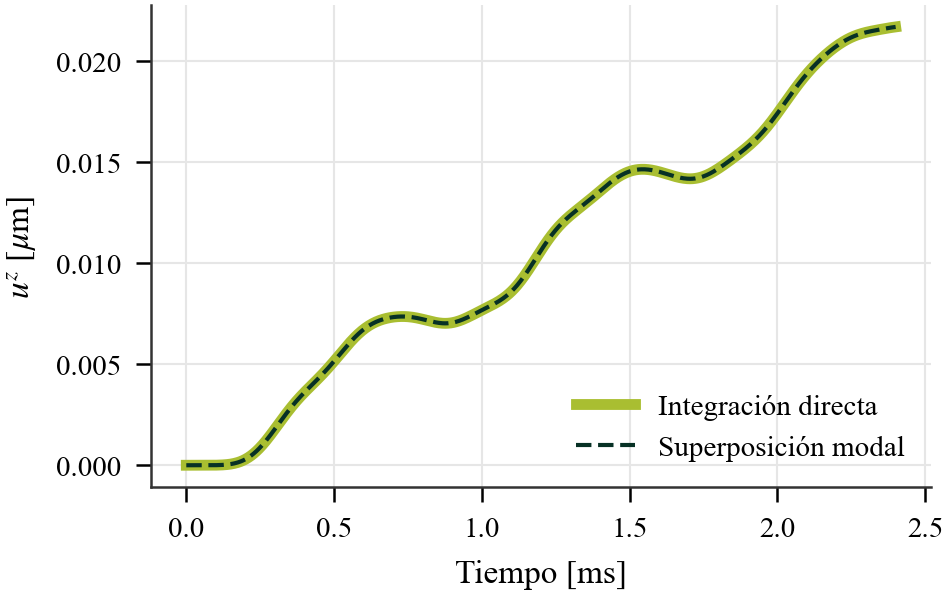
\includegraphics[width=\columnwidth]{fig15_validacion_modal_directa.png}
\caption{Desplazamiento transversal de un nodo calculado por superposición
modal y por integración directa con DOP853 en una red de prueba.}\label{fig:validacion}
\end{figure}

% =====================================================================
\section{Resultados y análisis}\label{sec:resultados}
% =====================================================================

\subsection{Configuración base y modos de vibración}

La \cref{fig:geometria} muestra la red base. La pretensión exterior,
$155.7\uN$, es del mismo orden que los $132\uN$ medidos por Lin y
Sobek~\cite{linsobek1998}, y la relación entre la pretensión radial media
y la masa de la araña, $\approx2\uN$/mg, está dentro del rango de 1.4 a
$7.2\uN$/mg medido por Wirth y Barth~\cite{wirth1992}. Toda la seda pesa
0.26~mg, unas 190 veces menos que la araña, así que la masa del sistema
está casi toda en el hub.

\begin{figure}[!htb]
\centering
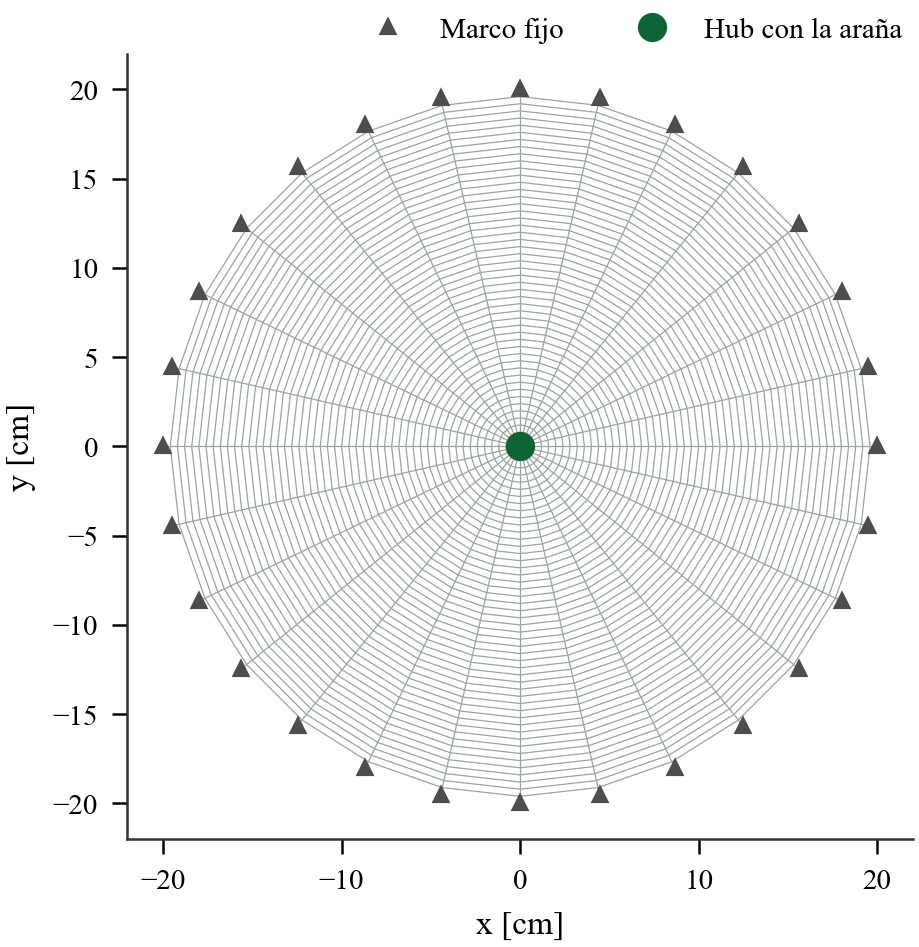
\includegraphics[width=\columnwidth]{fig01_geometria.png}
\caption{Red de la configuración base: 28 radiales, 49 anillos, hub libre
con la masa de la araña y marco fijo.}\label{fig:geometria}
\end{figure}

La familia transversal tiene 1373 modos, entre 2.55~Hz y 5.3~kHz, 191 de
ellos en la banda de 1 a 1000~Hz; la familia en el plano tiene 2746, entre
65.6~Hz y 196~kHz, 183 de ellos en esa banda. La \cref{tab:frecuencias} y
las \cref{fig:espectro,fig:p} resumen el espectro.

\begin{table}[t]
\centering
\caption{Primeras frecuencias naturales y número de onda azimutal $p$.}\label{tab:frecuencias}
\begin{tabular}{@{}ccc@{\hspace{1.5em}}ccc@{}}
\toprule%
\multicolumn{3}{c}{Transversales} & \multicolumn{3}{c}{En el plano}\\
Modo & $f$ [Hz] & $p$ & Modo & $f$ [Hz] & $p$ \\
\colrule%
1 & 2.554 & 0 & 1 & 65.577 & 1 \\
2 & 114.787 & 0 & 2 & 65.577 & 1 \\
3 & 130.265 & 1 & 3 & 130.265 & 0 \\
4 & 130.265 & 1 & 4 & 146.797 & 1 \\
5 & 162.003 & 2 & 5 & 146.797 & 1 \\
6 & 162.003 & 2 & 6 & 181.013 & 2 \\
\botrule%
\end{tabular}
\end{table}

\begin{figure*}[tb]
\centering
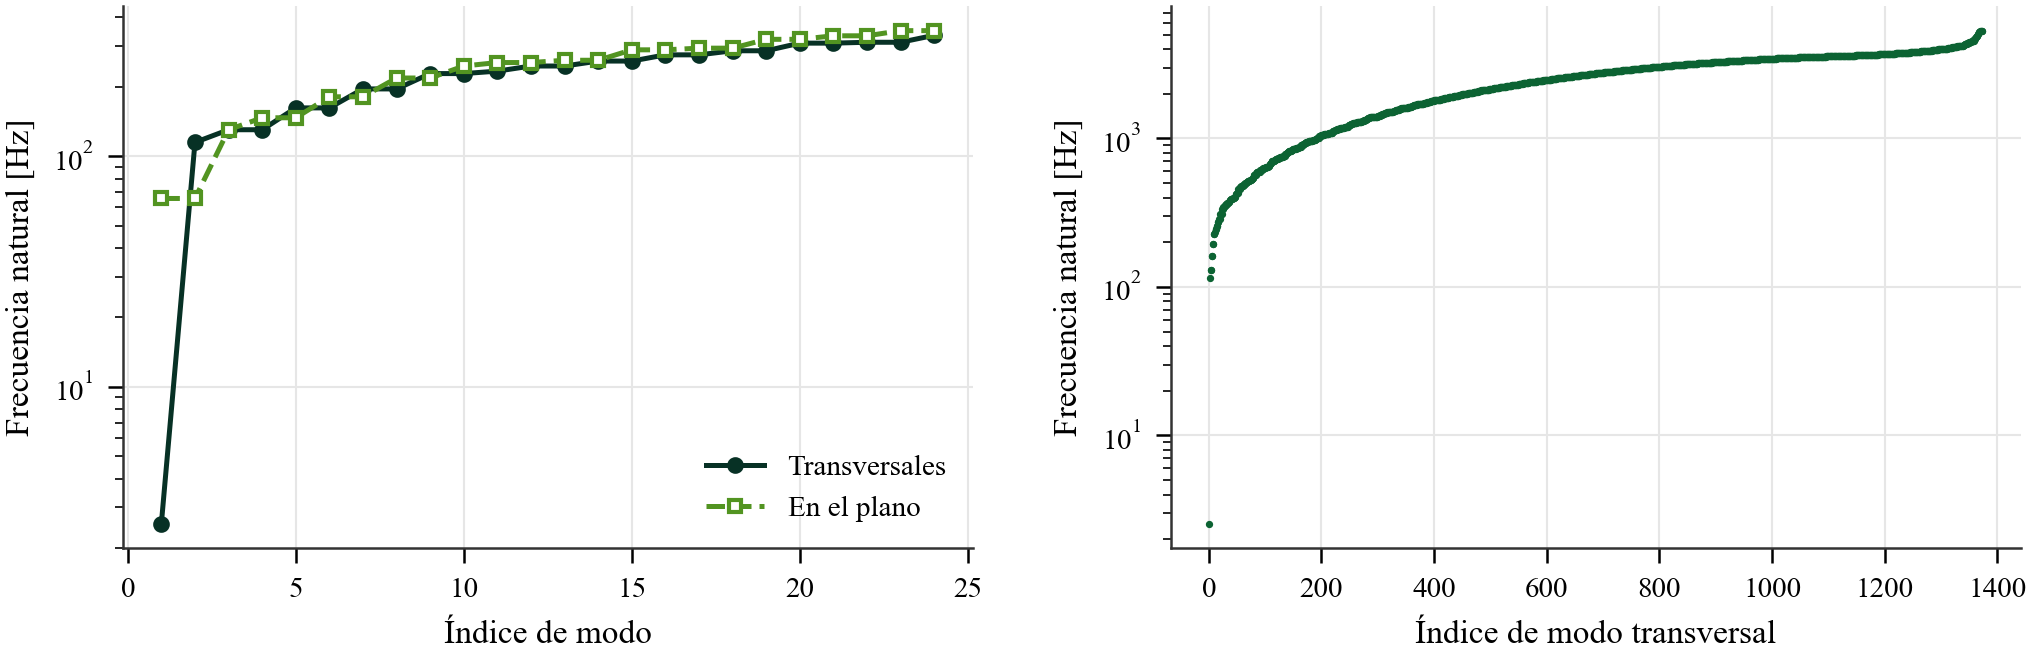
\includegraphics[width=\textwidth]{fig02_espectro_modal.png}
\caption{Espectro de frecuencias naturales. Izquierda: primeros 24 modos
de cada familia. Derecha: espectro transversal completo.}\label{fig:espectro}
\end{figure*}

\begin{figure}[!htb]
\centering
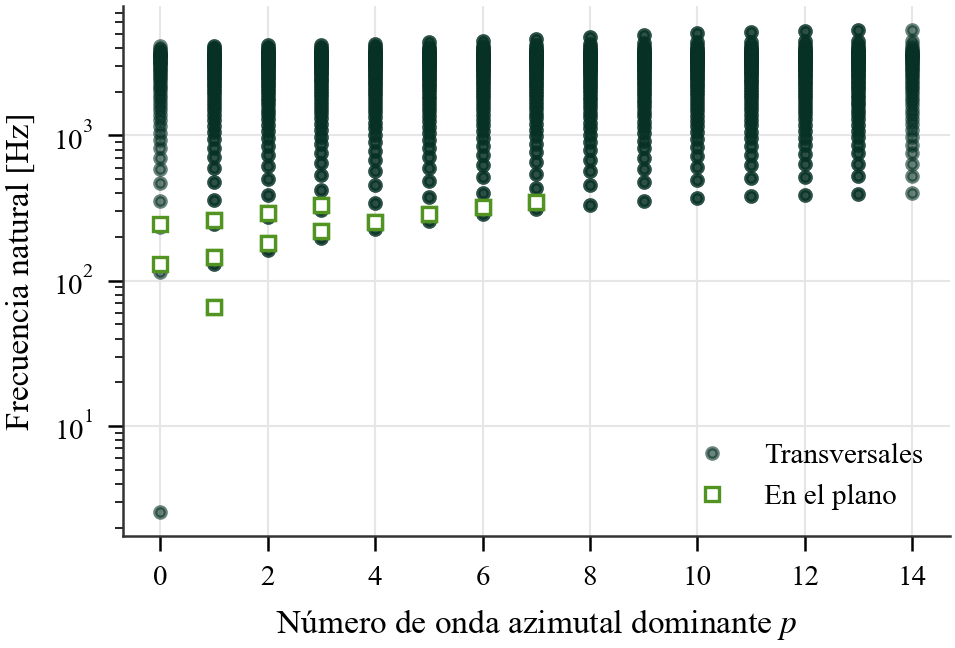
\includegraphics[width=\columnwidth]{fig03_frecuencia_vs_p.png}
\caption{Frecuencia natural de cada modo frente a su número de onda
azimutal dominante $p$.}\label{fig:p}
\end{figure}

El primer modo transversal, a 2.55~Hz y con $p=0$
(\cref{fig:modosT}), es el rebote de la araña: el hub sube y baja arrastrando a toda la red, con una
amplitud que decrece linealmente hacia el marco (\cref{fig:perfiles}). El
segundo, a 114.8~Hz y con $p=0$, es el modo fundamental de la red: todos los
radiales se mueven en fase mientras el hub permanece casi quieto por la
inercia de la araña. Los siguientes aparecen en pares de igual frecuencia,
a 130.3~Hz con $p=1$ y a 162.0~Hz con $p=2$, que corresponden a las dos
orientaciones, seno y coseno, de un mismo patrón.

\begin{figure*}[tb]
\centering
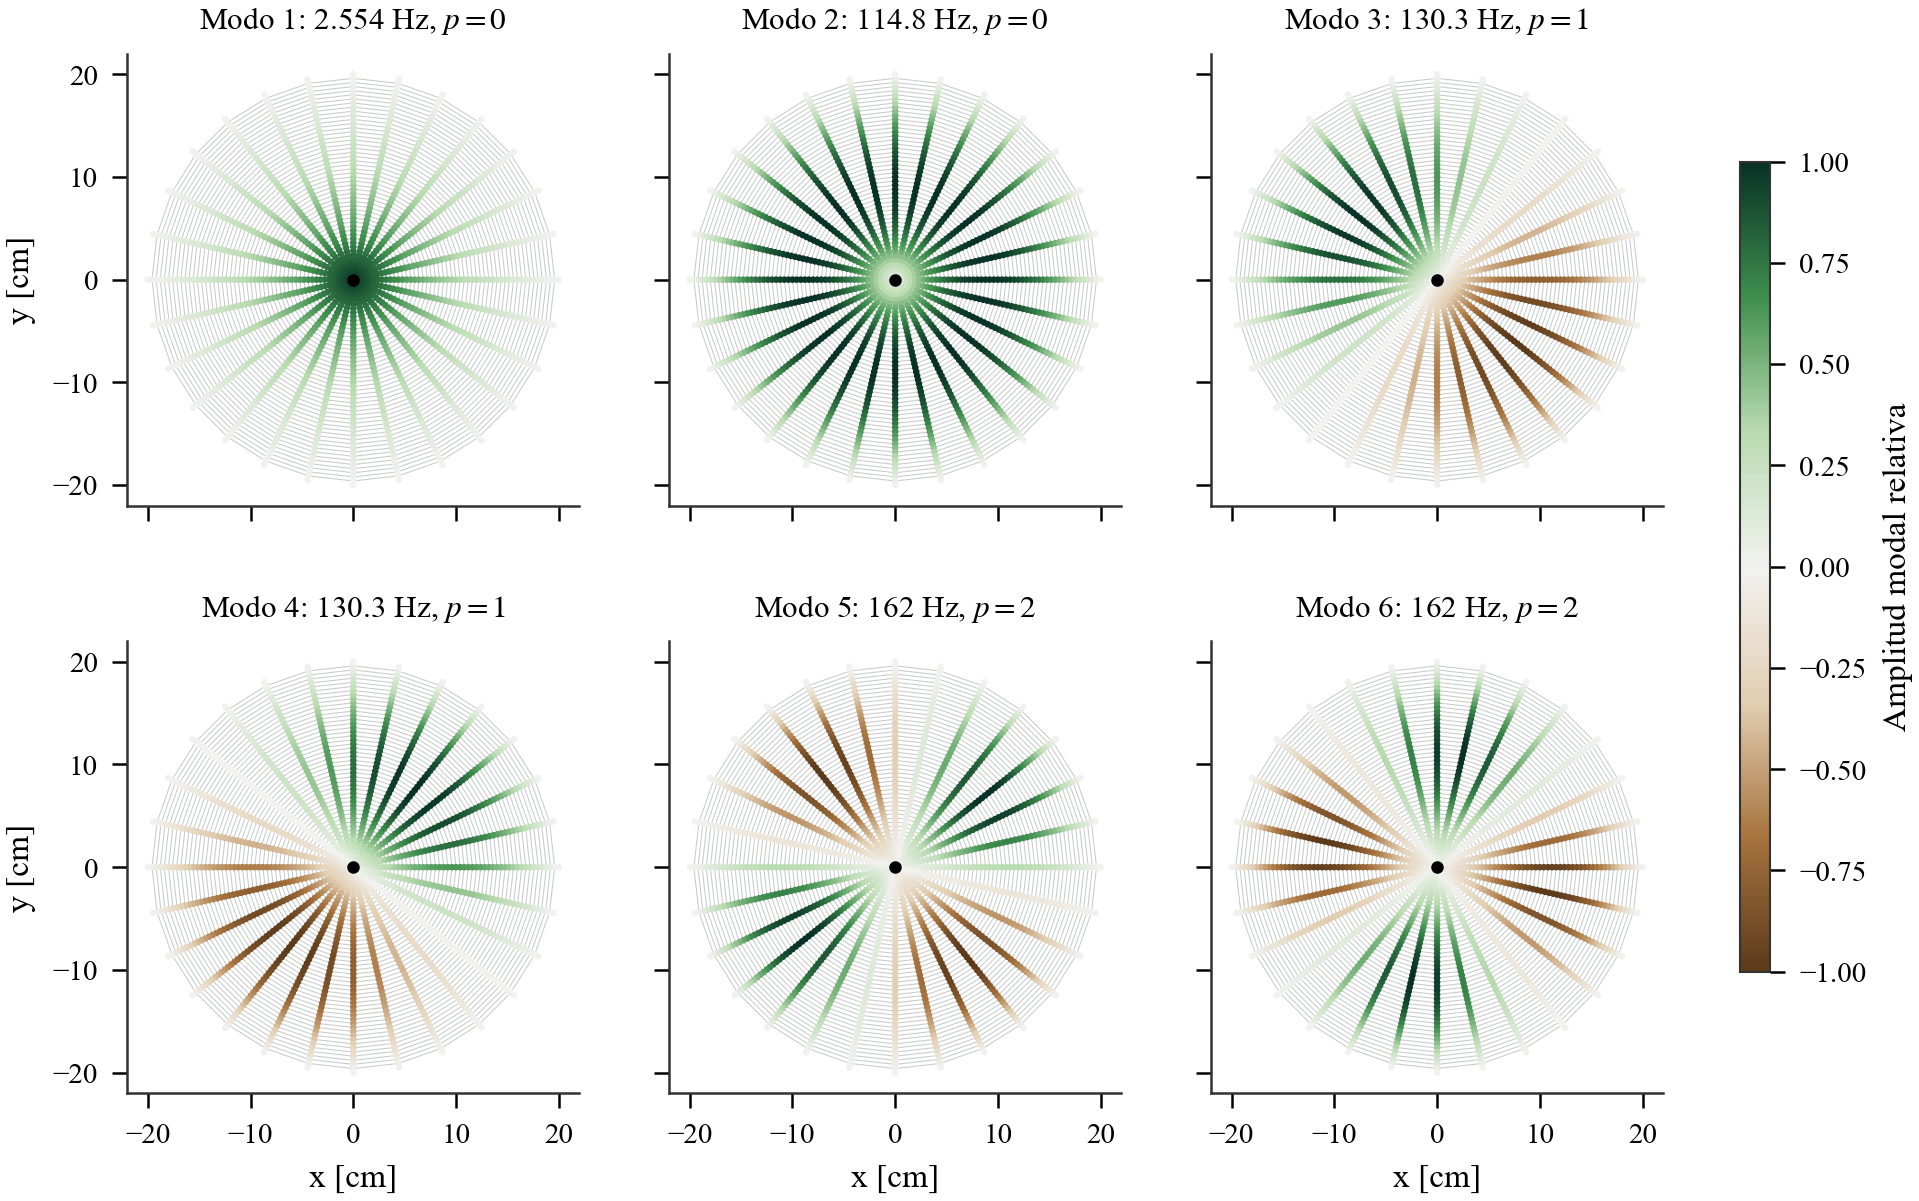
\includegraphics[width=0.7\textwidth]{fig04_modos_transversales.png}
\caption{Primeros seis modos transversales. El color indica la amplitud
modal relativa de la componente $z$: verde hacia arriba y marrón hacia
abajo.}\label{fig:modosT}
\end{figure*}

En el plano (\cref{fig:modosP}), el primer par, a 65.6~Hz y con $p=1$,
es la traslación de la araña dentro del plano, y el tercer modo, a
130.3~Hz y con $p=0$, una rotación de la red alrededor del hub.

\begin{figure*}[tb]
\centering
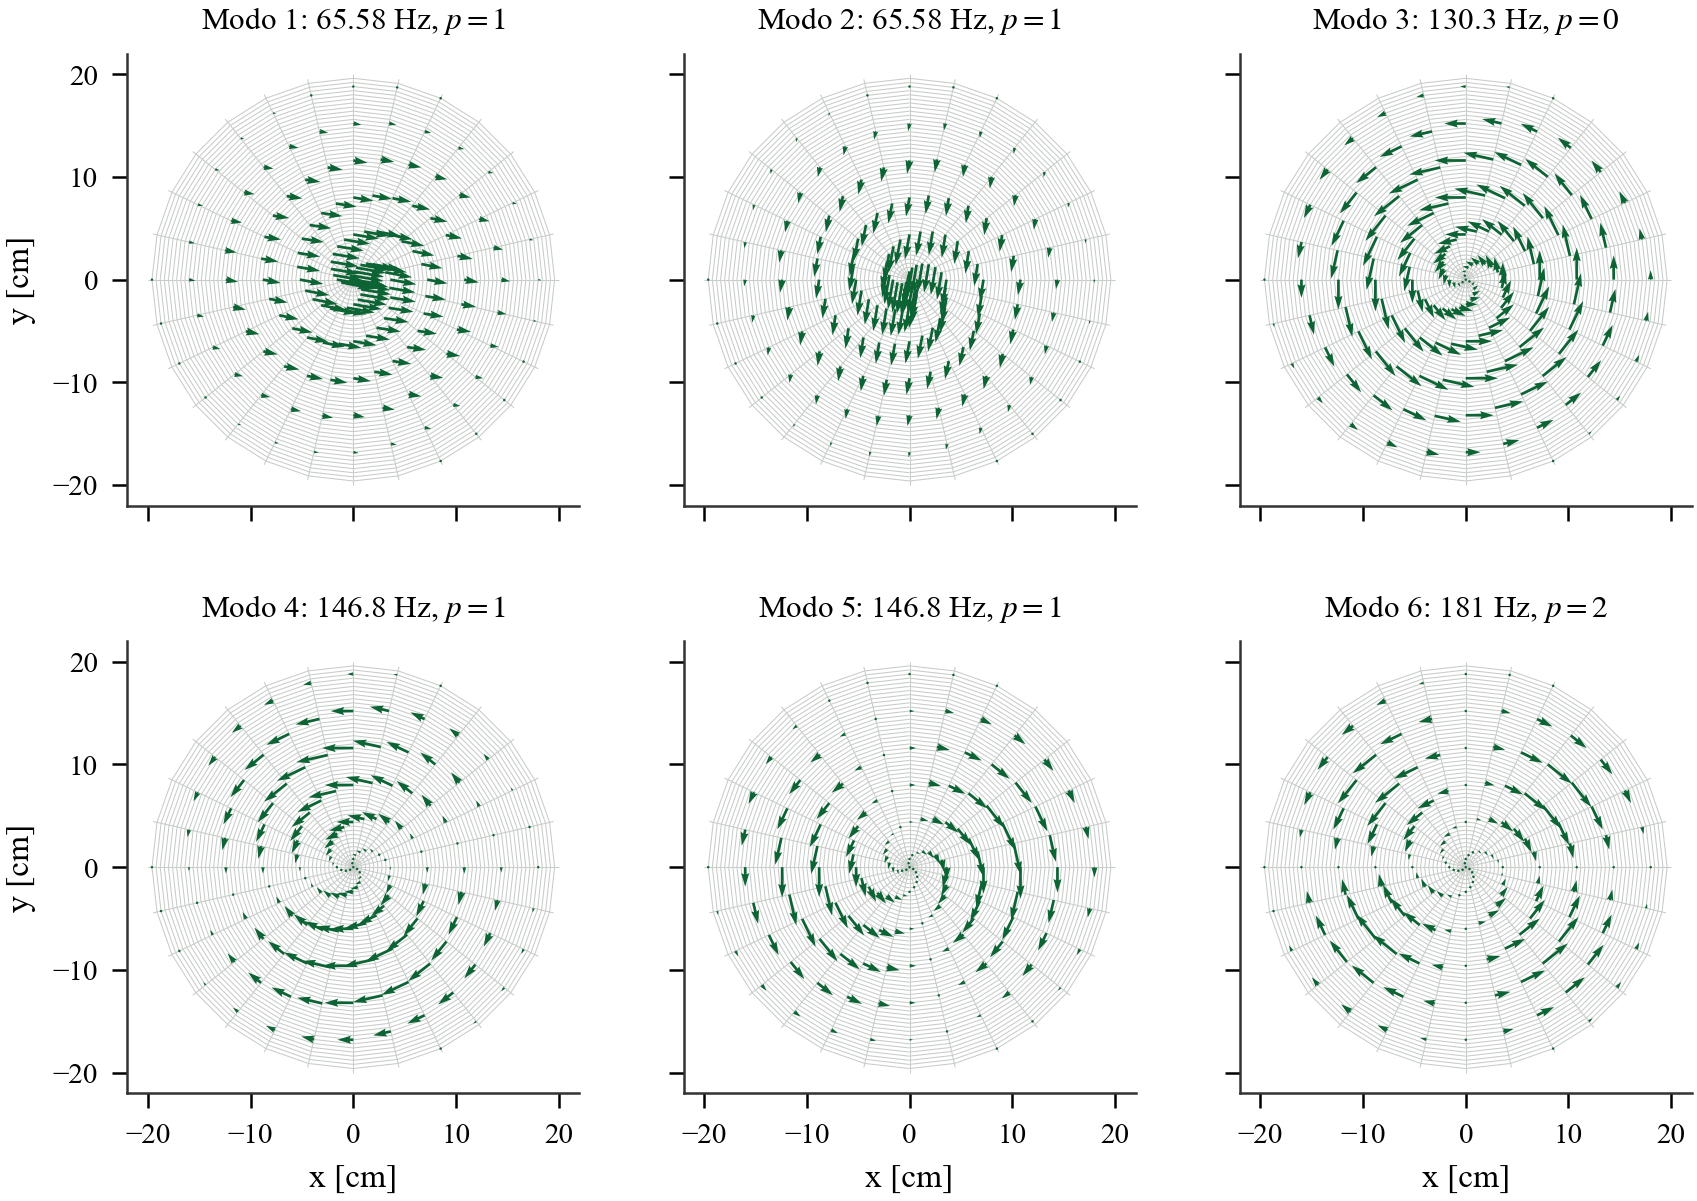
\includegraphics[width=0.7\textwidth]{fig05_modos_plano.png}
\caption{Primeros seis modos en el plano. Las flechas indican la dirección
y la amplitud relativa del desplazamiento $(u^x,u^y)$.}\label{fig:modosP}
\end{figure*}

\begin{figure}[!htb]
\centering
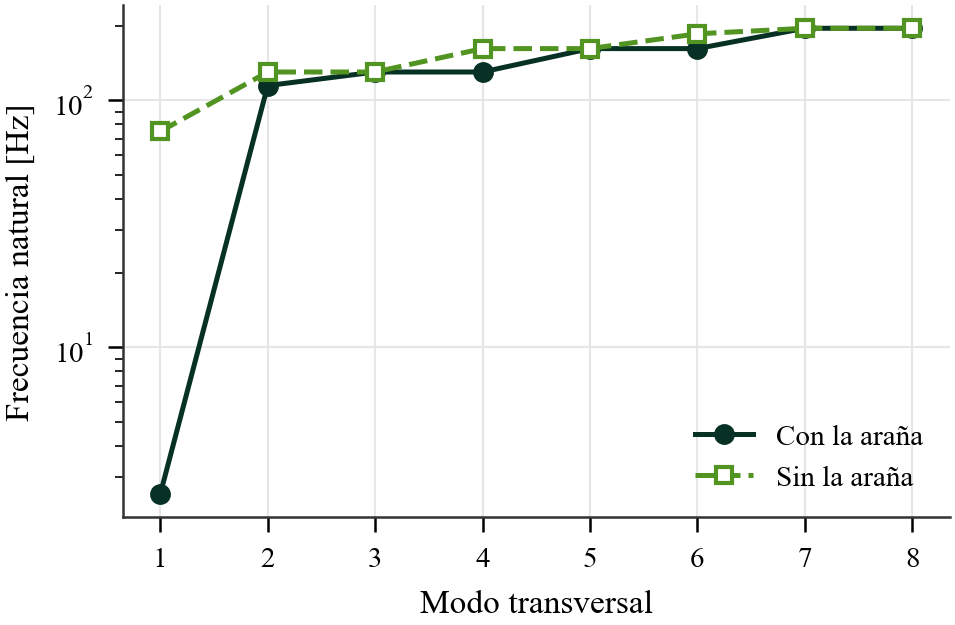
\includegraphics[width=\columnwidth]{fig06_comparacion_masa_arana.png}
\caption{Primeras frecuencias transversales con y sin la masa de la araña
en el hub.}\label{fig:masa}
\end{figure}

\begin{figure}[!htb]
\centering
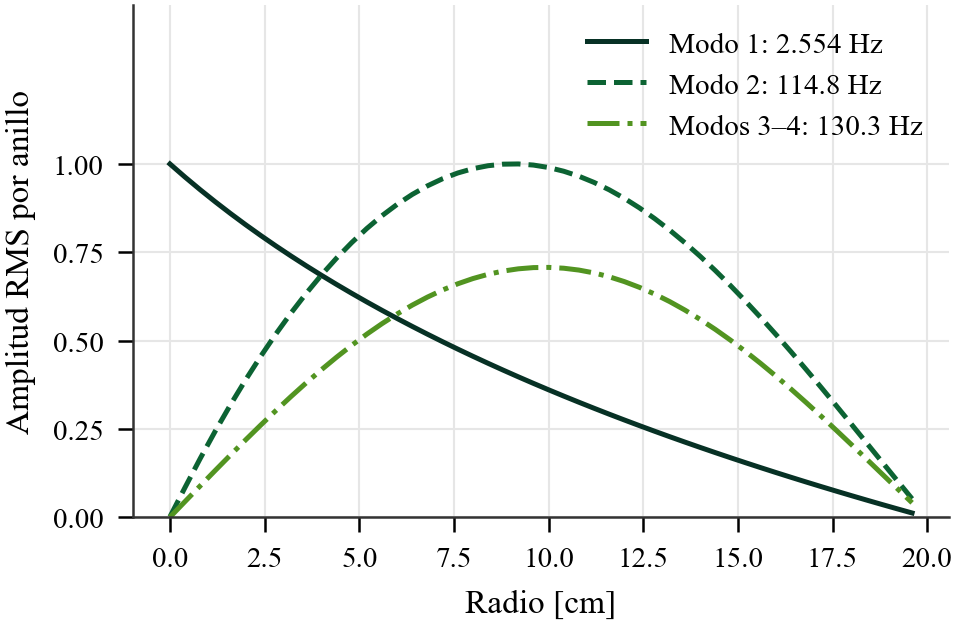
\includegraphics[width=\columnwidth]{fig07_perfiles_radiales.png}
\caption{Amplitud RMS por anillo de los primeros modos transversales. Los
modos 3 y 4 tienen el mismo perfil y sus curvas se superponen.}\label{fig:perfiles}
\end{figure}

\begin{figure}[!htb]
\centering
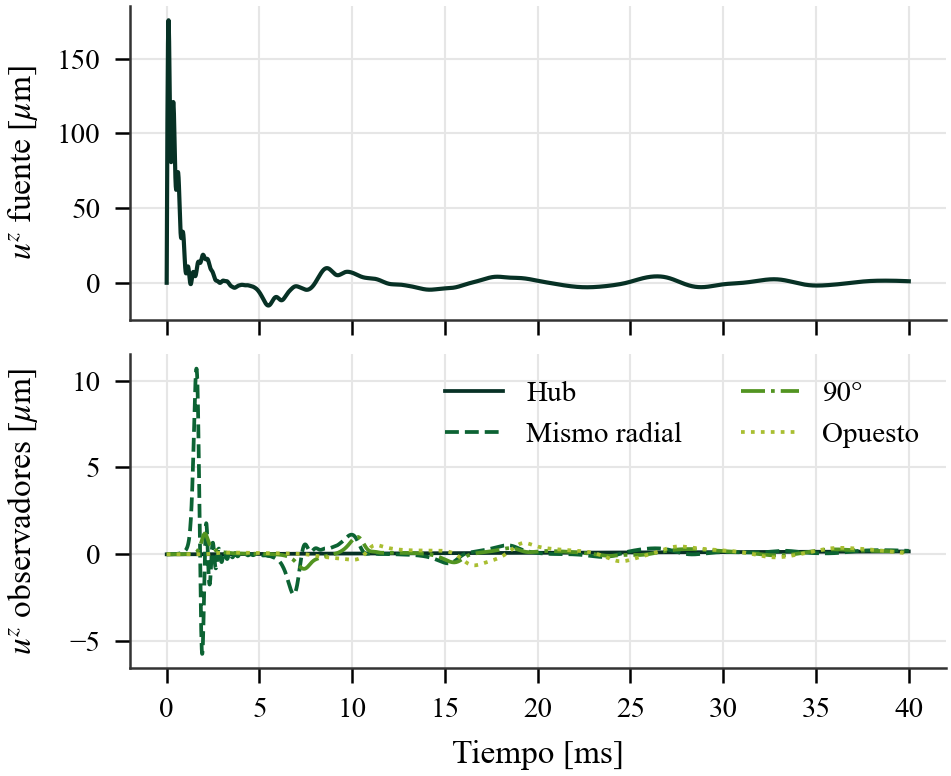
\includegraphics[width=\columnwidth]{fig08_respuesta_impulsional.png}
\caption{Desplazamiento transversal $u^z(t)$. Arriba, en la fuente;
abajo, en el hub y los tres observadores del anillo~1.}\label{fig:impulso}
\end{figure}

\begin{figure*}[tb]
\centering
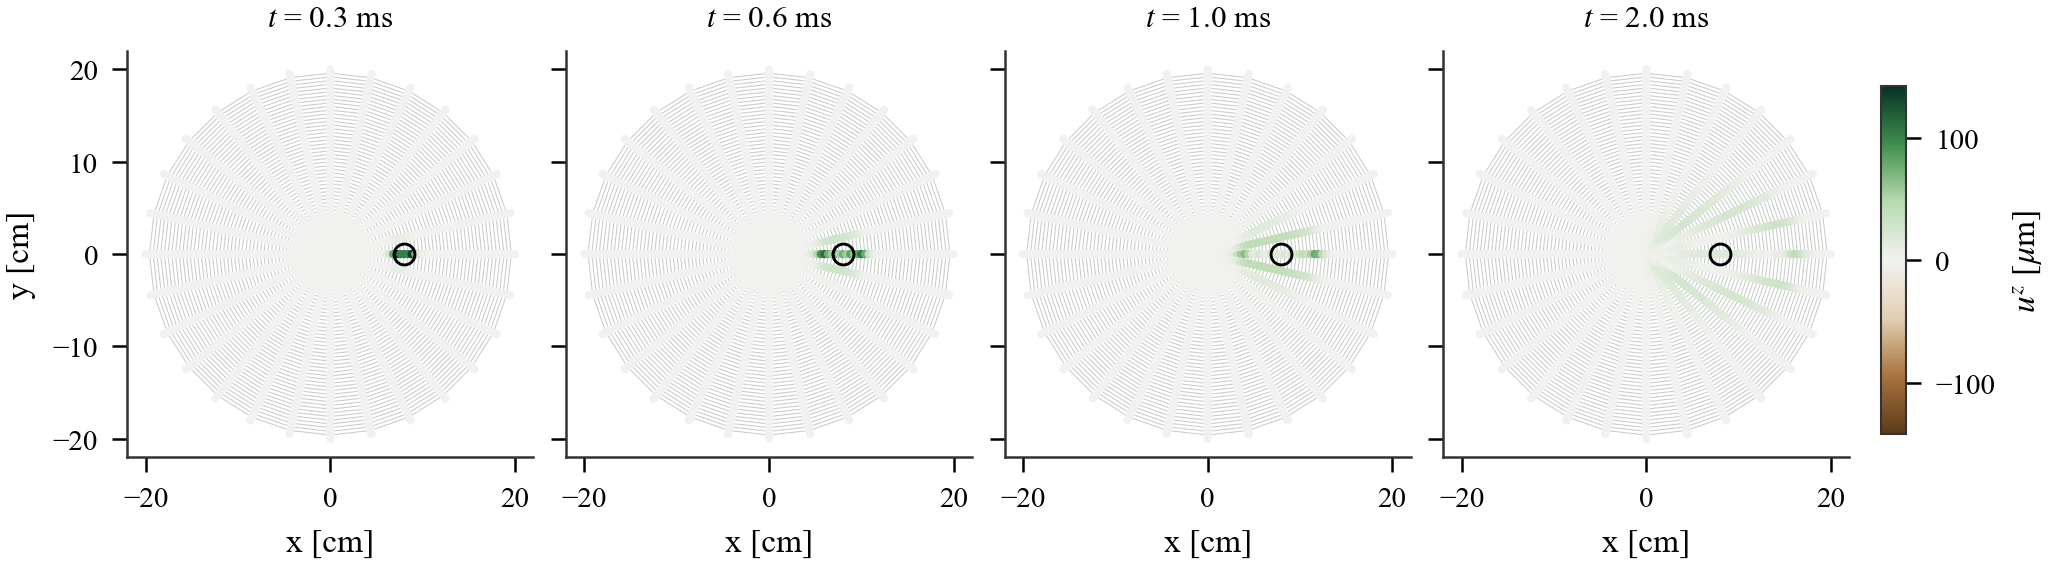
\includegraphics[width=\textwidth]{fig09_instantaneas_propagacion.png}
\caption{Propagación de la perturbación transversal en cuatro instantes,
con escala de color común. El círculo marca la presa.}\label{fig:snap}
\end{figure*}

\begin{figure}[!htb]
\centering
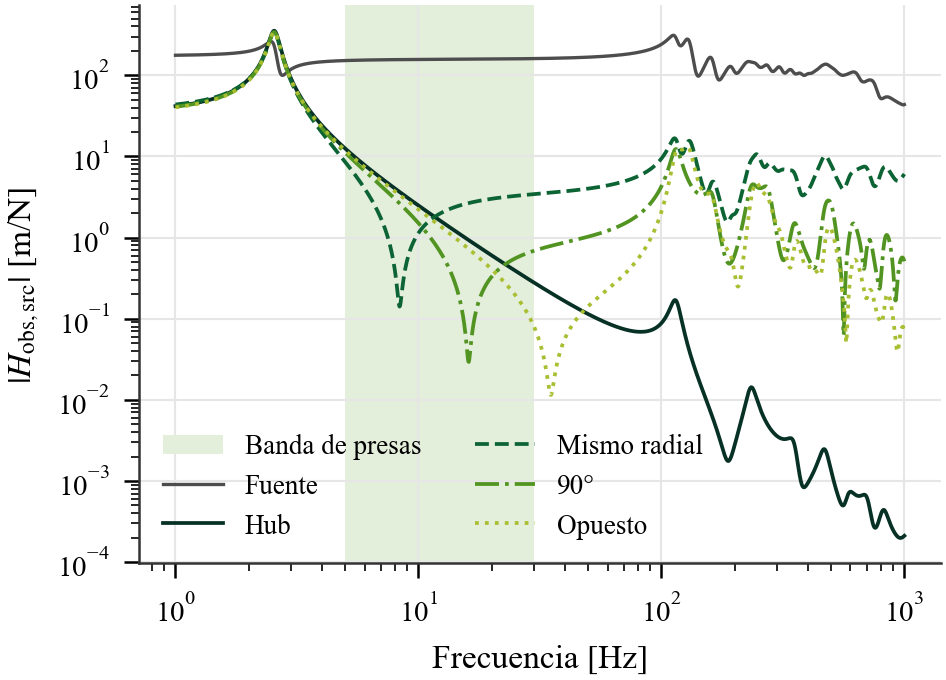
\includegraphics[width=\columnwidth]{fig10_funcion_transferencia.png}
\caption{Módulo de la receptancia $|H_{\mathrm{obs},\mathrm{src}}|$ entre
la presa y los observadores. La franja sombreada es la banda de presas,
de 5 a 30~Hz.}\label{fig:H}
\end{figure}

La masa de la araña es lo que más modifica el espectro (\cref{fig:masa}):
sin ella, la primera frecuencia transversal sube de 2.55 a 74.9~Hz y la
primera en el plano de 65.6 a 130.3~Hz, mientras que los modos con
$p\ge1$, en los que el hub no se mueve, no cambian. La araña no es, por
tanto, una corrección despreciable en la dinámica de baja frecuencia,
como ya anticipaban Frohlich y Buskirk~\cite{frohlich1982} para
frecuencias por debajo de unos 30~Hz.

\subsection{Respuesta a la perturbación de una presa}

En la fuente el desplazamiento alcanza $176\um$ a los 0.1~ms y decae en
unos 3~ms (\cref{fig:impulso}). La señal llega primero al nodo del
anillo~1 en el mismo radial, 1.2~ms después del impacto y con un pico de
unos $11\um$; a los radiales a $90^\circ$ y opuesto llega más tarde y con
alrededor de $1\um$, y el hub casi no se mueve en esos primeros
milisegundos. El frente viaja principalmente por el radial de la presa y
se reparte hacia los radiales vecinos a través de la espiral
(\cref{fig:snap}). Tomando como llegada a cada nodo el instante en que
$|u^z|$ supera el 5\,\% de su máximo, la velocidad aparente hacia el hub
es de 65~m/s, del mismo orden que la de una cuerda tensa,
$\sqrt{T^R/\lambda_{\mathrm{ef}}}\approx49$~m/s, con
$\lambda_{\mathrm{ef}}=\mu_i/\Delta$.

\subsection{Transmisión desde la presa hasta la araña}

La receptancia (\cref{fig:H}) tiene tres regiones. Cerca de 2.55~Hz todos
los observadores tienen el mismo pico, porque la red entera se mueve con
la araña. Entre 3 y 100~Hz no hay ningún modo transversal, así que la
respuesta es subresonante: cada observador sigue primero al hub y luego
presenta una antirresonancia, un mínimo en el que las contribuciones de
los modos se cancelan, a una frecuencia que crece con la distancia angular
a la presa: 8.4~Hz en el mismo radial, 16.1~Hz a $90^\circ$ y 35.1~Hz en
el opuesto. Por encima de 100~Hz aparecen las resonancias de la red.

\begin{table}[t]
\centering
\caption{Índice de transmisión normalizado
$\hat{\mathcal{T}}_{\mathrm{obs}}$ desde la presa en el nodo $(0,20)$.}\label{tab:T}
\begin{tabular}{@{}lcc@{}}
\toprule%
Observador & 1--1000~Hz & 5--30~Hz \\
\colrule%
Hub & $3.48\times10^{-3}$ & $3.27\times10^{-4}$ \\
Anillo 1, mismo radial & $6.26\times10^{-3}$ & $3.41\times10^{-4}$ \\
Anillo 1, a $90^\circ$ & $3.55\times10^{-3}$ & $2.16\times10^{-4}$ \\
Anillo 1, opuesto & $3.59\times10^{-3}$ & $2.81\times10^{-4}$ \\
\botrule%
\end{tabular}
\end{table}

\begin{figure*}[tb]
\centering
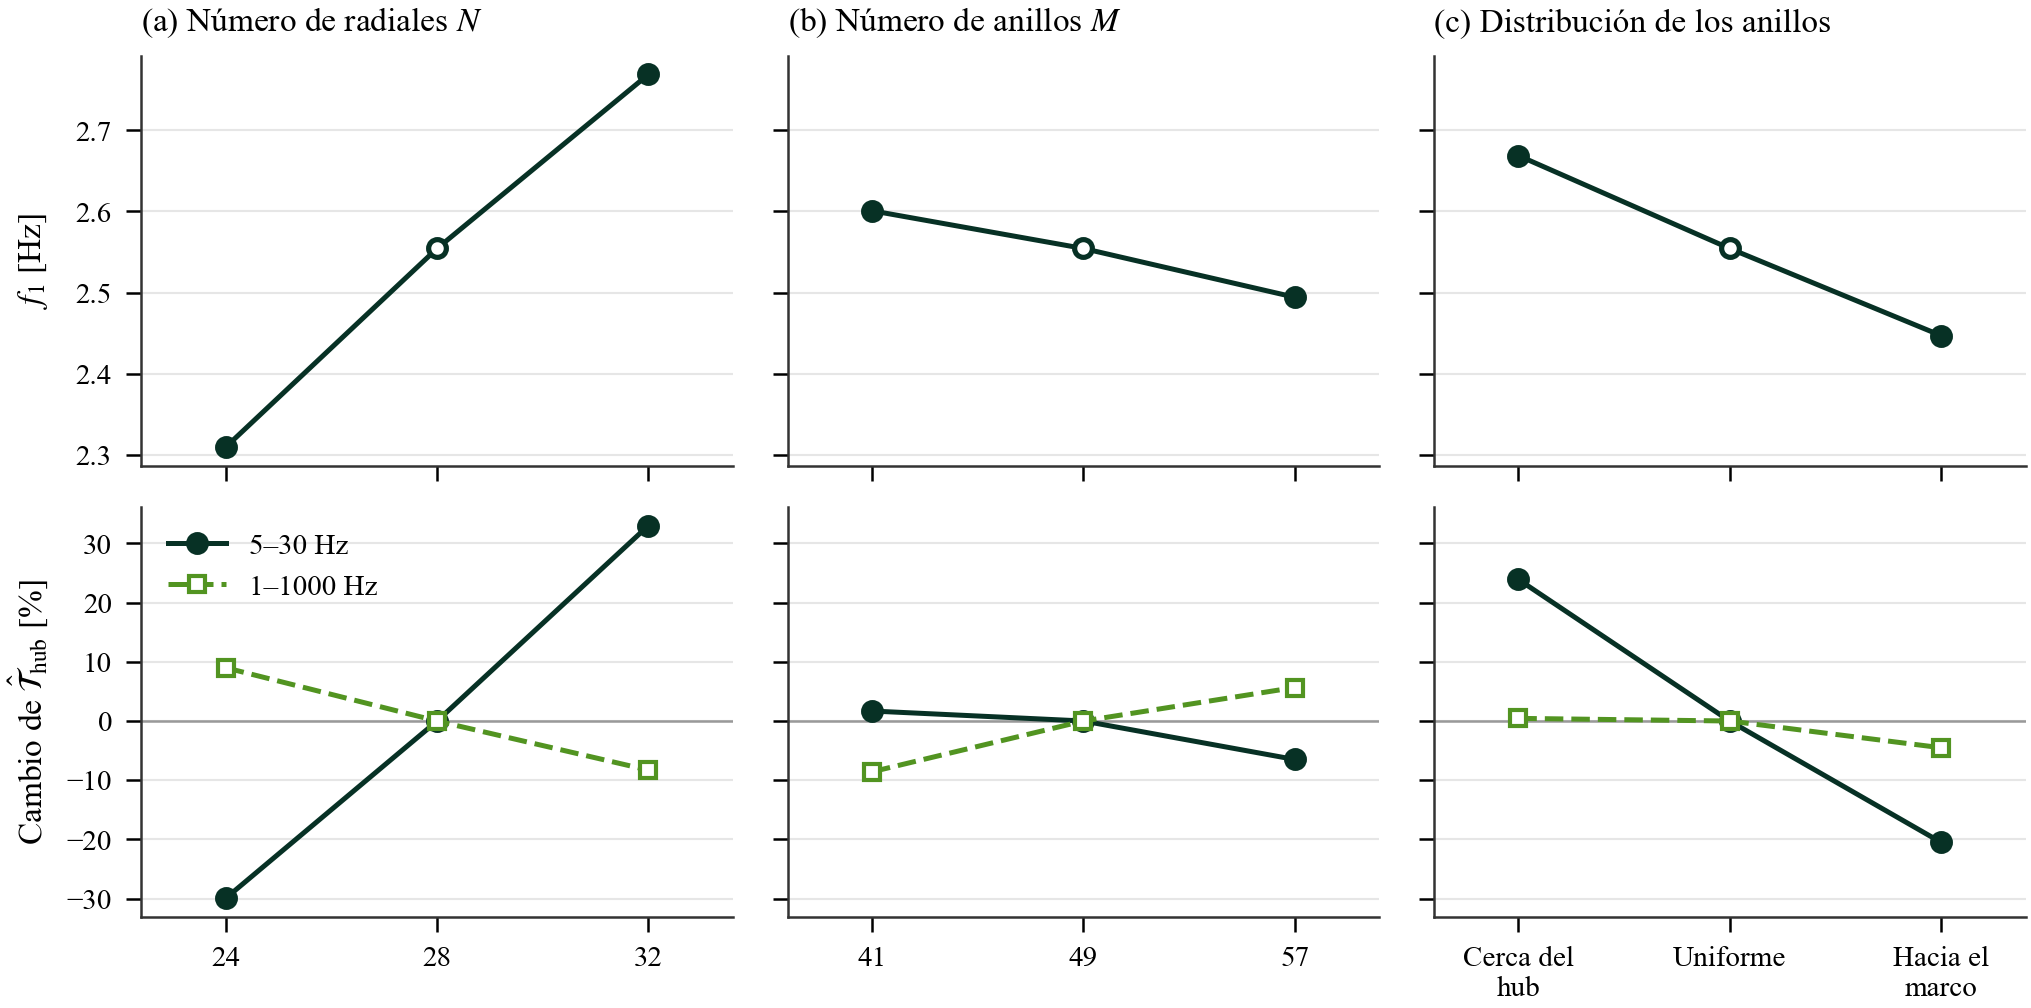
\includegraphics[width=\textwidth]{fig12_estudio_geometrico.png}
\caption{Efecto de la geometría. Arriba, primera frecuencia transversal;
abajo, cambio del índice de transmisión normalizado de la presa al hub
respecto a la configuración base, que es el punto central de cada
columna, en las dos bandas.}\label{fig:geo}
\end{figure*}

Según la \cref{tab:T}, los observadores del
anillo~1 reciben casi la misma señal integrada: el mismo radial recibe
1.8 veces más que los demás en la banda ancha y entre 1.2 y 1.6 veces más
en la de presas. Sin embargo, sí hay información direccional en la banda
de presas: a 30~Hz la receptancia hacia el mismo radial es 5 veces la del
radial a $90^\circ$ y 44 veces la del opuesto. El índice no la detecta
por dos razones: está dominado por el extremo inferior de la banda, de 5 a
8~Hz, donde todos los observadores se mueven con el hub, y los nodos del
anillo~1 están a solo 4~mm del centro, donde el movimiento del hub domina.

\begin{table}[t]
\centering
\caption{Cociente del índice de transmisión entre el observador del mismo
radial de la presa y los observadores a $90^\circ$ y opuesto, según la
distancia del observador al hub y la banda de integración.}\label{tab:direccion}
\begin{tabular}{@{}ccccc@{}}
\toprule%
 & \multicolumn{2}{c}{5--30~Hz} & \multicolumn{2}{c}{15--30~Hz} \\
Radio & $90^\circ$ & Opuesto & $90^\circ$ & Opuesto \\
\colrule%
0.4~cm & 1.6 & 1.2 & 45 & 59 \\
2.0~cm & 37 & 74 & 33 & 3950 \\
4.0~cm & 88 & 690 & 71 & 5220 \\
\botrule%
\end{tabular}
\end{table}

Para separar ambos efectos, la \cref{tab:direccion} repite el cálculo con
observadores a distintas distancias del hub y en la mitad superior de la
banda. A 2~cm del centro, una distancia comparable a la longitud de las
patas de la araña, el mismo radial recibe entre 37 y 74 veces más señal
que los demás en la banda de 5 a 30~Hz, es decir, entre 16 y 19~dB\@; el
contraste crece al alejarse del hub y al excluir las frecuencias más
bajas. Esto concuerda con Mortimer et al.~\cite{mortimer2019decoding},
quienes encontraron con un modelo de elementos finitos que comparar la
amplitud de la vibración entre las patas basta para determinar la
dirección de la presa. La información direccional está, entonces, en la
banda de presas, pero se pierde cerca del hub y en un índice que integre
toda la banda, donde domina el movimiento conjunto con la araña.

\subsection{Influencia de la geometría}

La \cref{tab:geometria} y la \cref{fig:geo} resumen el estudio
geométrico.

\begin{table*}[t]
\centering
\caption{Resultados del estudio geométrico. $f_1$ y $f_2$ son las dos
primeras frecuencias transversales, $f_1^P$ la primera en el plano y
$\hat{\mathcal{T}}_{\mathrm{hub}}$ el índice normalizado del hub. La fila
de la configuración base se repite en cada grupo.}\label{tab:geometria}
\resizebox{\textwidth}{!}{%
\begin{tabular}{@{}llcccccc@{}}
\toprule%
Variación & Configuración & $T^R_1$ [$\mu$N] & $f_1$ [Hz] & $f_2$ [Hz] & $f_1^P$ [Hz] & $\hat{\mathcal{T}}_{\mathrm{hub}}$, 1--1000~Hz & $\hat{\mathcal{T}}_{\mathrm{hub}}$, 5--30~Hz \\
\colrule%
Radiales & $N=24$ & 40.5 & 2.31 & 107.9 & 60.7 & $3.79\times10^{-3}$ & $2.29\times10^{-4}$ \\
 & $N=28$ (base) & 49.3 & 2.55 & 114.8 & 65.6 & $3.48\times10^{-3}$ & $3.27\times10^{-4}$ \\
 & $N=32$ & 55.9 & 2.77 & 120.5 & 70.1 & $3.19\times10^{-3}$ & $4.35\times10^{-4}$ \\
\colrule%
Anillos & $M=41$ & 58.0 & 2.60 & 122.5 & 65.6 & $3.18\times10^{-3}$ & $3.32\times10^{-4}$ \\
 & $M=49$ (base) & 49.3 & 2.55 & 114.8 & 65.6 & $3.48\times10^{-3}$ & $3.27\times10^{-4}$ \\
 & $M=57$ & 40.6 & 2.49 & 107.9 & 65.6 & $3.67\times10^{-3}$ & $3.05\times10^{-4}$ \\
\colrule%
Distribución & $\gamma=1.35$ (densa cerca del hub) & 49.3 & 2.67 & 122.7 & 65.6 & $3.49\times10^{-3}$ & $4.05\times10^{-4}$ \\
 & $\gamma=1$ (uniforme, base) & 49.3 & 2.55 & 114.8 & 65.6 & $3.48\times10^{-3}$ & $3.27\times10^{-4}$ \\
 & $\gamma=0.75$ (densa hacia el marco) & 49.3 & 2.45 & 109.2 & 65.6 & $3.32\times10^{-3}$ & $2.60\times10^{-4}$ \\
\botrule%
\end{tabular}}
\end{table*}

\textbf{Número de radiales.} De 24 a 32 radiales, la primera frecuencia
sube de 2.31 a 2.77~Hz y la señal que llega al hub en la banda de presas
aumenta un 90\,\% (\cref{fig:geo}a). Hay dos causas: más radiales
sostienen el hub y, según la \cref{eq:recurrencia}, con radiales más
cercanos entre sí la espiral tira menos hacia el centro, de modo que para
la misma pretensión media la pretensión junto al hub es mayor: $T^R_1$
pasa de 40.5 a $55.9\uN$. Como la rigidez transversal depende solo de
$T^0/L^0$ (\cref{eq:transversal}), ambos efectos rigidizan la zona donde
está la araña.

\textbf{Número de anillos.} Con más anillos todas las frecuencias bajan
(\cref{fig:geo}b); $f_2$ pasa de 122.5 a 107.9~Hz de 41 a 57 anillos.
Cada anillo añade masa de espiral y, de nuevo por la
\cref{eq:recurrencia}, reduce la pretensión junto al hub, que pasa de
58.0 a $40.6\uN$, porque el aumento total de la pretensión hacia afuera,
$2MT^S\sin(\pi/N)$, crece con $M$. La transmisión al hub en la banda de
presas solo disminuye un 8\,\%.

\textbf{Distribución de los anillos.} Concentrar los anillos cerca del
hub, con $\gamma=1.35$, sube las frecuencias y aumenta un 24\,\% la señal que
llega al hub en la banda de presas; concentrarlos hacia el marco la
reduce un 21\,\% (\cref{fig:geo}c). Como $N$, $M$ y las pretensiones no
cambian, la diferencia proviene de la masa: los anillos cercanos al
centro son más cortos, así que concentrarlos ahí reduce la masa total de
la espiral.

En conjunto, el
número de radiales es la característica que más modifica la transmisión
hacia la araña en la banda de presas, seguida por la distribución de los
anillos y, por último, por su número. Estos cambios, de decenas de por
ciento, son moderados frente al efecto de la masa de la araña sobre el
espectro o al de la posición del observador sobre la información
direccional.

\subsection{Rango de validez y limitaciones}\label{sec:validez}

Con el impulso usado, el hilo más exigido es el radial junto a la presa,
con $\delta_\perp/L=0.034$ frente al límite $2\sqrt{T^0/EA}=0.055$ de la
\cref{sec:justificacion}: el término despreciado alcanza el 40\,\% del
geométrico en el instante de máxima deformación. El modelo está, pues, en
el borde de su validez para esa amplitud, aunque esto solo afecta a las
amplitudes absolutas, ya que frecuencias, modos, cocientes de transmisión
y tiempos de llegada no dependen de $J$. En cuanto a las masas
concentradas, el primer modo interno de los radiales está por encima de
7~kHz, pero el de los tramos espirales de los anillos exteriores, de 9 a
20~cm del centro, está entre 470~Hz y 1~kHz. La banda de presas está bien
resuelta, pero por encima de unos 450~Hz el modelo omite modos de la
espiral; subdividir cada tramo espiral en varios elementos lo corregiría.

Además, solo se analizó la transmisión transversal, aunque las ondas en
el plano también informan sobre la dirección de la
presa~\cite{mortimer2019decoding}; la red es circular, horizontal y
simétrica, con marco rígido, mientras que las reales son verticales y
asimétricas~\cite{yavuz2024}, y no se incluye la masa del pegamento de
la espiral. Por último, $\zeta$ proviene de
ensayos cuasiestáticos, por lo que se usaron índices normalizados, y no se
dispone de una validación experimental propia.

% =====================================================================
\section{Conclusiones}\label{sec:conclusiones}
% =====================================================================

Se construyó un modelo lagrangiano de una telaraña orbicular que incluye
la rigidez elástica y la geométrica de los hilos. Se demostró que el
modelo está bien planteado cuando todos los hilos están tensos y la red
está anclada a un marco, y que el equilibrio de la red plana exige que la
pretensión radial crezca del centro hacia afuera. Para una red plana, los
movimientos transversal y en el plano se desacoplan de forma exacta, y las
vibraciones transversales dependen solo de las pretensiones, las
longitudes y las masas, que son justamente las variables que la araña
controla al construir la red. La implementación numérica se verificó con
las pruebas independientes de la \cref{tab:verif}; las comparaciones con soluciones exactas y
con la integración directa dan errores menores que $10^{-9}$.

Para \textit{A.~diadematus}, la masa de la araña, 190 veces mayor que la
de la seda, domina la dinámica de baja frecuencia: produce un modo de
rebote a 2.55~Hz, frente a 74.9~Hz sin ella, y deja la banda de vibración
de presas, de 5 a 30~Hz, entre ese modo y el fundamental de la red, a
114.8~Hz. En esa banda la respuesta es subresonante y cada observador
tiene una antirresonancia que depende de su posición respecto a la presa.
La información sobre la dirección de la presa está en esa banda, pero
solo a cierta distancia del hub: a 2~cm del centro el radial de la presa
recibe entre 37 y 74 veces más señal que los demás, mientras que a 4~mm el
movimiento del hub la oculta.

De las características geométricas estudiadas, el número de radiales es
la que más modifica la señal que llega a la araña, con un aumento del
90\,\% al pasar de 24 a 32 radiales, seguida por la distribución de los
anillos, que la cambia un 20\,\%, y por su número, que la reduce un
8\,\%. Una parte importante del
efecto de la geometría no es directa, sino que actúa a través de las
pretensiones que impone el equilibrio. La geometría modifica la respuesta
de forma moderada en comparación con la masa de la araña y con la
posición en la que se mide la señal.

Como trabajo futuro se propone estudiar la transmisión en el plano,
subdividir los tramos espirales para resolver frecuencias por encima de
450~Hz, incluir la masa del pegamento y la asimetría de las redes
verticales, y contrastar el modelo con mediciones experimentales.

% ---------------------------------------------------------------------
% Referencias
% ---------------------------------------------------------------------
\bibliographystyle{jaes}
\bibliography{referencias}

\end{document}
